\subsection{Otros problemas al extraer información}

En algunos de los problemas que surgieron, encontramos detalles particulares que tuvimos que resolver caso por caso. Ésto para poder guardar la información de manera adecuada. A continuación se presentan los diferentes casos encontrados:
  
  \begin{itemize}
\item[-] Dentro de la obtención de datos del número de alumnos, no se lee la información cuando se tiene \textit{``Un alumno''}, ya que no se reconoce el texto \textit{``Un''} como el número $1$. En la \figurename{~\ref{UnAlumno}} vemos un ejemplo de este caso: \url{http://www.fciencias.unam.mx/docencia/horarios/20081/119/1809}.

\begin{figure}[H]
\centering

\includegraphics[scale = 1]{Ej_un_alumno} %width=\textwidth
\caption[\textit{Grupo con un alumno}]{\textit{Se muestra un ejemplo de grupo con el texto ``Un'' y no el número $1$.}}\label{UnAlumno}
\end{figure}

Para resolver este problema se identificó la variable tipo \textit{string} igual a \textit{``Un''} para convertir la información y así poder utilizar los datos obtenidos.

\item[-] El algoritmo supone que todas las clases duran una hora y no se consideran las medias horas. En la \figurename{~\ref{MediasHoras}} mostramos un ejemplo: \url{http://www.fciencias.unam.mx/docencia/horarios/20172/1556/820}. Se considera que esa materia inicia a las 18hrs.

\begin{figure}[H]
\centering
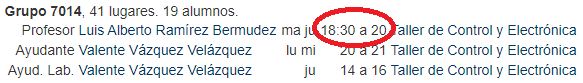
\includegraphics[width=\textwidth]{Ej_gpo_medias_hrs} %scale = 0.9
%\url{http://www.fciencias.unam.mx/docencia/horarios/20172/1556/820}
\caption[\textit{Grupo con medias horas}]{\textit{Se muestra un ejemplo de grupo con medias horas. Se considera que las materias inician en horas enteras y no a las medias horas.}}\label{MediasHoras}
\end{figure}

\item[-] Se tienen materias con múltiples horarios. En estos casos sólo se registran los horarios y salones en los que los profesores imparten su clase, no se toman en cuenta las clases impartidas por los ayudantes.

En la \figurename{~\ref{horariosMultiples}} tenemos un ejemplo de este caso: \url{http://www.fciencias.unam.mx/docencia/horarios/20181/2055/1323}. El profesor imparte su clase los lunes, miércoles y viernes de 13-14hrs en el salón O215, hay una ayudantía los martes y jueves de 13-14hrs en el salón O215 y otra ayudantía los martes de 11-13hrs en el salón 304 (Yelizcalli). Se considera que esta materia inicia a las 13hrs y se imparte en el salón O215.

\begin{figure}[H]
\centering

\includegraphics[width=\textwidth]{Ej_gpo_horarios_multiples} %scale = 0.8
\caption[\textit{Grupo con horarios múltiples}]{\textit{Se muestra un ejemplo de grupo con horarios múltiples. En estos grupos sólo se toman en cuenta los horarios y salones en los que los profesores imparten clase.}}\label{horariosMultiples}
\end{figure}

\item[-] Las materias de inglés no se imparten todos los días de la semana, en algunos casos se imparten clases en línea. Se registran únicamente los horarios de los días en que se imparten las clases presenciales. En la \figurename{~\ref{casoIngles}} mostramos un ejemplo de este caso: \url{http://www.fciencias.unam.mx/docencia/horarios/20202/2017/1135}.

\begin{figure}[H]
\centering

\includegraphics[scale = 1]{Ej_gpo_ingles} %width=\textwidth
\caption[\textit{Grupo de inglés}]{\textit{Se muestra un ejemplo de un grupo de inglés. Las clases no se imparten todos los días. Hay sesiones virtuales. Sólo se toma en cuenta el horario de las clases presenciales.}}\label{casoIngles}
\end{figure}

\item[-] Se tienen grupos que no tienen la misma estructura que los tipos de grupos \textbf{A}, \textbf{B} y \textbf{C} definidos en la Sección \ref{TiposDeGpos}, debido a ello el código CSS utilizado no sirve para extraer toda la información que se puede obtener del grupo. En la \figurename{~\ref{GpoEstructuraDiferente}} tenemos un ejemplo de este caso en donde no se lee adecuadamente el número de alumnos inscritos en el grupo: \url{http://www.fciencias.unam.mx/docencia/horarios/20201/2017/872}.

\begin{figure}[H]
\centering

\includegraphics[width=\textwidth]{Ej_gpo_con_estructura_diferente} %scale = 0.8
\caption[\textit{Grupo con estructura diferente}]{\textit{Se muestra un ejemplo de grupo con estructura diferente. En estos casos no se extrae adecuadamente la información de los grupos porque el código CSS utilizado no corresponde a este tipo de grupos.}}\label{GpoEstructuraDiferente}
\end{figure}

\end{itemize}